\documentclass[a4paper,10pt]{article}
\usepackage[english]{babel}
\usepackage[utf8]{inputenc}
\usepackage[toc,page]{appendix}
\usepackage{graphicx}
\usepackage{multirow}
\usepackage{array}

%Includes "References" in the table of contents
\usepackage[nottoc]{tocbibind}
\usepackage{titling}
\usepackage{setspace}




\parskip 1ex

%\setlength{\droptitle}{-10em}
%\setlength{\topmargin}{-0.2in} % was -1

\usepackage{fancyheadings}
\usepackage{ifthen}
\usepackage{titlesec}
%\setlength{\textheight}{9in} %was 10.2

%Begining of the document
\begin{document}
	
	\title{\textbf{CSCM35: Big Data and Data Mining \\Coursework 2}}
	\date{01/05/20}
	\author{Andy Gray\\445348}
	
	\maketitle
	\begin{center}
		\item
\includegraphics[width=9cm]{swansea.png}
	\end{center}
	
	\thispagestyle{empty}
	\newpage
	\pagenumbering{arabic}
	
	\section{Introduction}
	
	%\small 
	We have presented upon us a challenge to complete a practical data mining task, which involves a technical report and a software solution. We have a dataset provided that has been collect by Johns Hopkins CSSE in real-time, with values related to the current pandemic the coronavirus (COVID-19) \cite{jhmcdata}. However, we need to use additional datasets to complete complement the provided data. Once identifying a research question, we need to develop a prototype and evaluate our method. 
	
	With the COVID-19 first declaring over 800 cases on the 23rd of January 2020, and figures still rising, which at point of writing was 3.12m cases and 217K deaths worldwide \cite{worldmeter}, the virus has reached over 199 different countries. We wanted to see if between the time scale of the 22nd of January and the 25th of April, what is the general public sentiment is. We want to know, has the general public sentiment changed, or if it has stayed the same? While over the COVID-19 pandemic.
	
	We will first achieve this by using Twitters API to gain all the tweets that have been tweeted, over this time, using the hashtag' coronavirus'. We will then complete a sentiment analysis on the data, to gain an overall view of the general feel of the 'coronavirus' tweets. Gaining the sentiment value will allow us to have insights into the public view, and if these tweets are positive or negative and how they change as the pandemic plays out over time. 
	
	The sentiment analysis showed that the sentiment value has been moving in a negative direction from January to April. However, when looking at the months individually, January and February, at the beginning of the declaration of the pandemic, Twitter's tweets had a slight positive sentiment at the beginning, then quickly declined into a negative sentiment. March had a very positive start to the month, then had a massive drop to negative figures in the middle of the month to return positive to then return slightly in the negative numbers at the end of the month. April started negative, with a small positive spike to carry on the negative downward trajectory.
	
	The report will first explain our proposed solution. Explaining how we aim to get the tweets from Twitter, and then put the contents into a CSV file. We then will explain how we intend to use the Natural Language Toolkit (NLTK) to train our classification models. We will then explain how we intend to provide the classifiers with the extracted tweets and gain a sentiment score based on the content of the tweets. We will then explain the packages used and describe the dataset and any preprocessing techniques we used. We will then explain the results which are then followed by a discussion on the results and a conclusion.
	
	\section{Proposed Solution}
	We will be using Twarc, a Python library for archiving Twitter JSON data. The library accesses the Twitter API to extract a JSON object as Twitter stores tweets as line-oriented JSON. The Twarc library handles the Twitters's API, as well as its rate limits. This library also allows us to use hydrate tweet ids. It is collecting the relevant tweet's details that match the criteria of having hashtags of 'coronavirus' \cite{twarc}.
	
	We will then use another python library called hydrate. Hydrate allows us to be able to take the Tweet ID's that we have taken off twitter, by using Twarc and get the contents of the actual tweet. Hydrate will provide us back with the content of the tweet, along with other potentially crucial information. We only need for this sentiment analysis the values "created\_at" and "full\_text". Once the tweets get collected for all of the Tweet IDs, we will then convert the JSON data into a CSV file. We will then do sentiment analysis on the tweets to gauge the over feel of these tweets. To see if they are all negative or if they overall a positive vibe over each day.
	
	We will then use NLTK to create a sentiment analysis on the tweets text body. However, before we could do this, we needed to use several packages to get a trained model, to provide us with the likelihood of the tweet being positive or negative. To classify the tweet, we used SKLearn's Naive Bayes MultinomialNB and BernoulliNB, Linear Model's LogisticRegression, SGDClassifier and SVM's SVC, LinearSVC, NuSVC. We then used NLTK's ClassifierI and SKLearnClassifer modules for carrying out the classification of the words process. 
	
	We then create a sentiment function, which takes in a parameter of text. This function will find the features of the parameter and then return the classification of the tweet if it was positive or negative, and the confidence level of that tweet with its analysis. The value we pass the function is the tweets 'full\_text' value. The classification and confidence level gets outputted as a .txt file.
	
	%[Do I use a stage to tidy up the data as there is so much? -> If so explain here]
	
	To visualise the data, we use Matplotlib and the outputted .txt to populate the graph. We are displaying the sentiment values of the tweets, allowing us to see the trend in the tweets sentiment analysis. 
	
	
	\subsection{Packages}
	%Need to update.
	We used Python 3 \cite{Python} as our programming language as it allowed us to use the required libraries and additional pages we needed. One of the main libraries was NLTK, a leading platform for building programs to work with human language \cite{nltk}. SKLearn \cite{van2014scikit} for its Naive Bayes, linear model and SVM libraries. Along with Statistics for its mode library. Altair and Matplotlib \cite{hunter2007matplotlib} were used to visualise the data. We used Pickle \cite{Python} to handle the saving and loading of the trained classifiers for the sentiment analysis program. 
	
	
	%We will be using the programming language Python 3 \cite{Python}, as this allows us to use all the required additional packages needed. The additional packages we will be using are NumPy \cite{walt2011numpy}, OpenCV \cite{opencv_library}, Pptk, Matplotlib \cite{hunter2007matplotlib}, SKImages \cite{van2014scikit}, SKLearn \cite{sklearn_api} and Tensorflow version 2 \cite{tensorflow2015-whitepaper}.
	
	\subsection{Dataset and Preprocessing}
	%The presented dataset provided, which is maintained by Johns Hopkins CSSE, consists of [decsribe data here]. The data had many missing values, which correlate to the country not having any COVID-19 cases, so these features got filled in with zeros.
	
	The presented dataset provided, which is maintained by Johns Hopkins CSSE, consists of data from the world and their COVID infected and death rates. The data had many missing values, which correlate to the country not having any COVID-19 cases, so these features got filled in with zeros. This dataset got used initially to paint an overall picture of the COVID situation around the world. However, it did not get used for any of the sentiment analysis.
	
	With using Twarc, we were able to gain 23.462 million tweets. Twarc was able to pull 1.857 million tweets between 22/01/20 to 28/02/20, 9.367 million between 01/03/20 to 31/03/20 and 12.238 million unique tweets between 01/04/20 to 25/04/20.
	
	Through using Twarc and Hydrate, we had to drop features from the table that were not required. The required features we needed were 'created\_at' and 'full\_text'.
	
	In order to train our sentiment analysis models, we used a sample .txt file that contained positive text, and another .txt file that contained negative text. Along with NLTK's class FreqDist, we were able to encode the frequency distributions. The frequency distribution counts the number of times an experiment has that outcome occur \cite{nltkfreqdist}.
	
	\subsection{Sentiment Analysis}
	Sentiment analysis is a type of data mining. Sentiment analysis is a form of semi-supervised machine learning \cite{tan2016introduction, geron2019hands} which uses classification, a text-based classification approach \cite{jingjingslidesNLP}. It aims to measure what the inclination of people's opinions is, through using natural language processing (NLP). It can also get referred to as Society text data mining \cite{jingjingslidesNLP}. NLP is a computational linguistics and text analysis. It gets used to extract and analyse information from the Web, which is mostly social media and other similar sources. The analysed data quantifies the general public's sentiments or reactions toward certain situations, products, people or ideas and reveal the contextual polarity of the information. Sentiment analysis is also known as opinion mining \cite{towarddatasciencesentiment}.
	
	Sentiment analysis can fall into two categories, pure statistics or a mix of statistics and linguistics \cite{towarddatasciencesentiment}. Pure statistics use algorithms like the Bag of Words (BOW). This kind of algorithms filters the text down to only the words that the algorithm believes to have sentiment, taking into account no context to the sentence at all. Such models do not aim to understand the language, only analyse the statistical measures to classify the text. 
	
	The mix of statistics and linguistics approach uses an array of Natural Language Processing (NLP) techniques, along with statistics to allow the machine to understand the language truly. The algorithms achieve this by incorporating languages grammar principles into analyst of the text. 
	
	There are broadly two main outputs to sentiment analysis. One type of sentiment analysis output gets referred to as Categorical/Polarity. What this means is that the text will get classed as either positive, negative or neutral overall. While the other is Scalar/Degree. What this means is that a score is given based on a predefined scale, that ranges from highly positive to highly negative. This type of sentiment analysis output has been used on tweets to see the views on various USA election candidates.
	
	For this experiment, we will use the purely statistical approach to gauge if a tweet that we gather off twitter is positive or negative.
	
	%For this experiment, we will use the purely statistical approach to gauge if a tweet that we gather off twitter is positive or negative.
	
	\section{Results}
	
	%\begin{figure}[t]
	%	\label{confusion_matrix}
	%	\small
	%	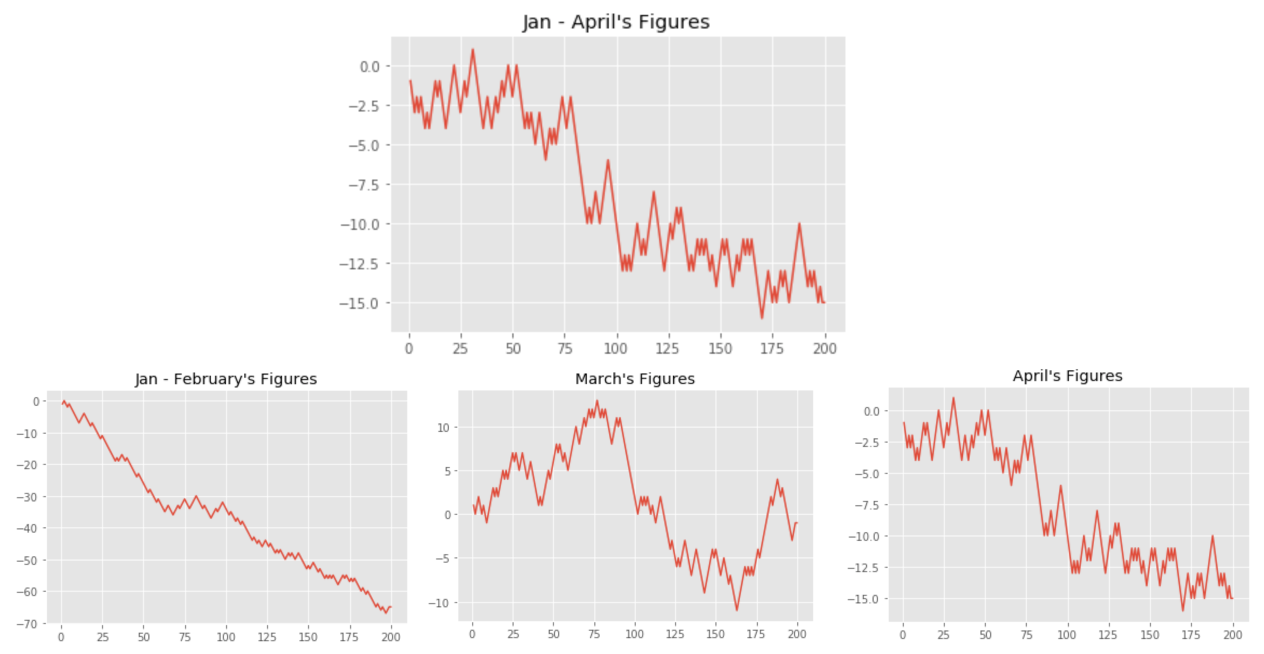
\includegraphics[width=8cm]{results.png}
	%	\\Fig \ref{confusion_matrix}: This is the confusion matrix from the 3x3 and 6x6 filter training.
	%	\centering
	%\end{figure}
	
	\begin{center}
		\label{confusion_matrix}
		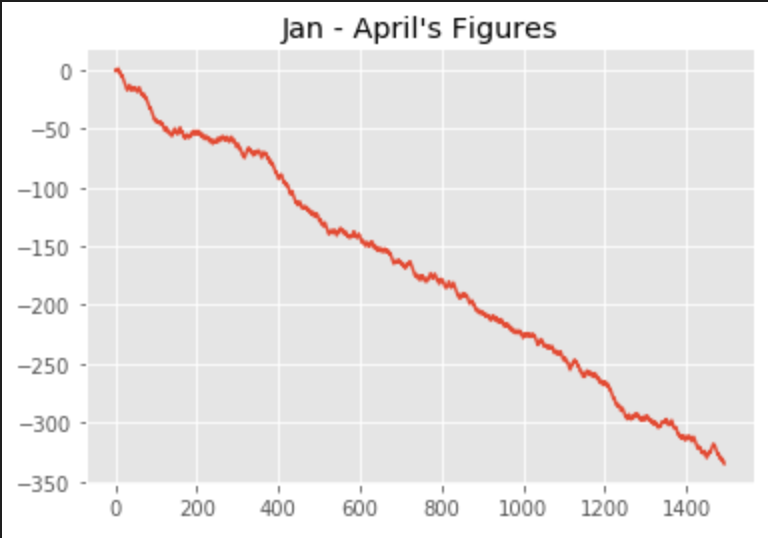
\includegraphics[width=8cm]{allresults2.png}
		\centering
		\\Fig: These graphs show the sentiment analysis for January 23rd to April 25th. 
	\end{center}

	The results show that a negative trend has been happening since the 23rd of January. Furthermore, although the values have been going in a negative direction, There have been occurrences where there has been more positive in sentiment, showing that it is not all doom and gloom. However, not enough to take the value back over zero and into the positive figures. The highest gaining ~2 which the lowest value being ~-325.
	
	\begin{center}
		\label{confusion_matrix}
		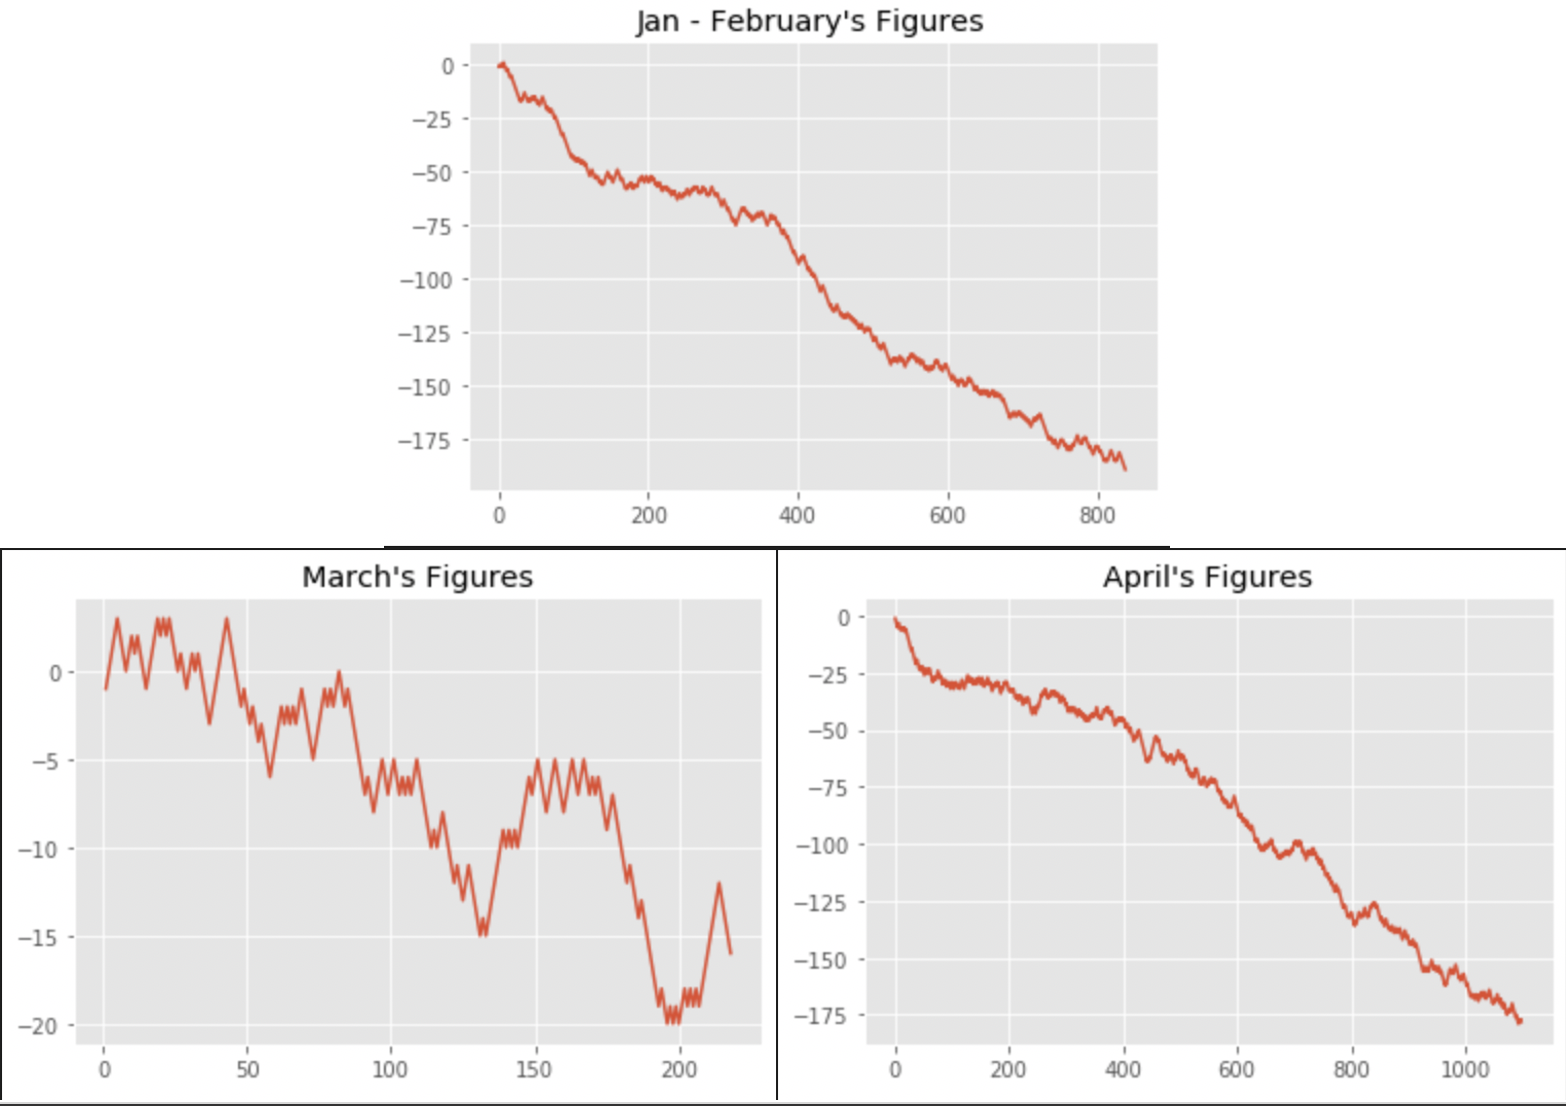
\includegraphics[width=12cm]{eachmonth3.png}
		Fig:  These show each months sentiment analysis individually.
	\end{center}

	As we can see from January to February tweet sentiment analysis table, the values start to go in a positive direction but quickly move down into a negative position. With the occasional spike in the tweets positivity, however, not enough to stop the downward trend, ending the month on a value lower than ~-180. 
	
	On the other hand, March had much more of an up and down result. In terms of the moods over the month, it went from extreme positive at the beginning to a sharp decline, to then return positive to go back slightly negative at the end of the month. The highest positive value was ~15, while the lowest value was ~-20. It was showing that the month overall had more positive tweets than negative.
	
	April's analysis shows that the month started in a negative place and continued the downward trend then. With the highest positive value being ~0 while the lowest value being ~-175.5.
	
	\section{Discussion}
	
	Understandably, January and February had a negative trajectory as this was the moment in time that the WHO was declaring the pandemic. Which naturally causes fear and confusion about what is in store for us with this virus. However, March started on a very positive trend, but that quickly started to go on a negative trajectory. It would be interesting to see what correlations can get made to what caused the positive start, could this be linked to the positive news coming out about people recovering and surviving? It is also interesting to see the steep negative trajectory as well, could this be linked to when most of the western worlds went into lockdown, as we have gained mainly English speaking nations tweets, who went into lockdown around the 23rd of March.
	
	With the proposed solution only looking at words, a pandemic like we are currently in would have a lot of negative words get used which could result in the tweet getting seen as negative. However, if the context of the tweet gets taken into full account then the tweet itself might not be negative, just containing many words, that on their own and taken out of context, could be perceived as negative.
	
	In regards to the sentiment analysis checking the tweets that contain the hashtag 'coronavirus', it does provide a limited scope. It would be good to be able to compare the results against other hashtags of a similar nature. For example, on the hashtags 'covid-19', 'virus', 'covid', 'ncov19' and 'ncov2019'. Have these hashtags overall had more of positive sentiment or even been used more due to the smaller size in word count?
	
	\section{Conclusion}
	We have found after gaining tweets from Twitter, that contained the hashtag 'coronavirus', between the dates of the 23rd of January to the 25th of April, we can see that the overall sentiment analysis value has been moving in a negative direction. Therefore, Showing us that the overall mood towards to Corona Virus is a very negative one. However, when we look at the months individually, March has a very positive start, but then quickly dropped into negative figures, to then recover and return to the middle, on more of negative learning though.
	
	April also had a positive spike at the beginning of the month, but then continued on the negative trajectory. We speculate that the positive was on the build-up to the western worlds declaring 'Social Distancing', and the sharp decline the after marks. However, further studies need investigating to conclude this hypothesis. Furthermore, trying to establish what was happening, at the time, to cause the positive trends in the trajectory within the different months.
	
	Overall we feel that this gives a good insight into the mood and feelings of society, that uses Twitter. However, we do feel that using additional similar hashtags, that are maybe shorter in length due to Twitter's word limit in tweets, would allow us to have a better understanding of the overall picture. Rather than just using the one hashtag.
	
	
	%\medskip
	\newpage

	\bibliographystyle{acm}
	
	{\footnotesize
		\bibliography{samples}
	}
	
	
\end{document}